\documentclass[a4paper,12pt]{report}

\usepackage[utf8]{inputenc}
\usepackage[french]{babel}
\usepackage[T1]{fontenc}
%\usepackage[scaled]{helvet} % police
\usepackage{lmodern}
\usepackage{layout}
\usepackage[top=2cm, bottom=1.5cm, left=2cm, right=2cm]{geometry}
\usepackage{setspace}
\usepackage{verbatim}
\usepackage{moreverb}
\usepackage{listings}
\usepackage{graphicx}
\usepackage{shorttoc}
\usepackage{xcolor}
\usepackage{currfile}
\usepackage{hyperref}

\setcounter{topnumber}{4}
\setcounter{bottomnumber}{4}
\setcounter{totalnumber}{10}
\renewcommand{\textfraction}{0.15}
\renewcommand{\topfraction}{0.85}
\renewcommand{\bottomfraction}{0.70}
\renewcommand{\floatpagefraction}{0.66}

%\include{chapterStyle}

\makeatletter
\def\thickhrulefill{\leavevmode \leaders \hrule height 1ex \hfill \kern \z@}
\def\@makechapterhead#1{%
  \vspace*{10\p@}%
  {\parindent \z@ \raggedleft \reset@font
            \scshape \@chapapp{} \thechapter
        \par\nobreak
        \interlinepenalty\@M
    \Huge \bfseries #1\par\nobreak
    %\vspace*{1\p@}%
    \hrulefill
    \par\nobreak
    \vskip 20\p@
  }}
\def\@makeschapterhead#1{%
  \vspace*{10\p@}%
  {\parindent \z@ \raggedleft \reset@font
            \scshape \vphantom{\@chapapp{} \thechapter}
        \par\nobreak
        \interlinepenalty\@M
    \Huge \bfseries #1\par\nobreak
    %\vspace*{1\p@}%
    \hrulefill
    \par\nobreak
    \vskip 20\p@
  }}

\renewcommand\thesection{\arabic{section}}
%\renewcommand*\familydefault{\sfdefault} %% Only if the base font of the document is to be sans serif


% Redéfinition de commandes

% Pour avoir les noms de chapitre en 1.1.3 etc...
\renewcommand\thesection{\arabic{chapter}.\arabic{section}}

% Désactiver les alinéas automatiques
%\parindent=0cm


% Création du glossaire

\setcounter{tocdepth}{4}

\begin{document}
  \begin{onehalfspace}

  % Page de garde
    \begin{titlepage}
      \begin{center}
        Sébastien Corbin et François-Guillaume Ribreau\\
        CSII 2\ieme année\\
        Le 21 Septembre 2011\\
      \end{center}
      \hrulefill
      \vspace{7cm}
      \begin{center}
        \LARGE \textbf{Dossier de conception}\\
        \vspace{3cm}
        \normalsize Génie Logiciel Embarqué
      \end{center}

      \vspace{9,5cm}

      \begin{center}
      \line(1,0){250}
      \end{center}

      \begin{center}
      \tiny{\currfilename}
      \end{center}


    \end{titlepage}
    \clearpage

  \thispagestyle{empty}
  \setcounter{page}{0}
  \clearpage

\chapter{Objectifs du système}
L'objectif de ce projet est de fournir une application mobile destinée à exploiter une plateforme d'application géo-localisée.

\chapter{Interfaces}
\section{Interfaces Utilisateurs}
L'application GeoBBS est conçue pour être utilisée sur un téléphone mobile iPhone.
Cette interface utilisateur a été amplement décrite dans le dossier de spécifications dans lequel vous retrouvez tous les détails nécessaires à la compréhension de cette interface.
Cette application mobile va donc être utilisée pour l'exploitation du projet GeoBBS et son accès est protégé par le couple login / mot de passe.

\section{Interfaces Logicielles}
Les interfaces logicielles mentionnées ici sont des interfaces internes au système.

\begin{description}
  \item[Interface avec la base de données centrale]: l'application doit interagir avec la base de données centrale (MongoDb, installée sur le serveur de base de données) au moyen de pilotes dédiés, de manière synchronisée. Cette base de données rassemble toutes les données manipulées par l'application.

\end{description}

\section{Interfaces de communication}
  Les interfaces de communication mentionnées ici sont des interfaces internes au système.

  \begin{description}
    \item[Interface entre l'application mobile et le serveur]: pour accéder aux données et aux services présentés par l'application mobile, une connexion TCP/IP est nécessaire.
  \end{description}

\chapter{Bases de données externes}
  Aucune base de données externe n'est prévue pour interagir avec notre système. Les seules bases de données, mentionnées précédemment, font partie du système à concevoir.

\chapter{Contraintes générales de conception}
  Plusieurs contraintes provenant de différentes sources sont à prendre en compte dans la phase de conception du système. Ci-dessous, un récapitulatif des contraintes imposées par le cahier des charges :

\begin{itemize}
  \item Le framework PanicAR doit être utilisée pour la création de l'écran utilisant la réalité augmentée.
  \item La base de données doit être de type MongoDB. La base de données doit être synchronisée à intervalle régulier avec l'application mobile.
  \item La phase de conception n'est démarrée qu'après validation du modèle métier (et du modèle conceptuel des données) par le maître d'ouvrage.
  \item L'application doit être en anglais. Le code en anglais.
\end{itemize}

\chapter{Documents de référence}
.

\chapter{Normes, Standards et Outils}

\subsection{Méthodes de conception}
  Les méthodes de conception sont utilisées afin d'améliorer la qualité de la conception finale.

\begin{itemize}
\item La méthode de conception MERISE a été utilisée pour mettre en place le Modèle Métier du système,  le  Modèle Conceptuel de Données (MCD), le  Modèle Logique de Données (MLD)  pour aboutir enfin au script de génération de la base de données.

\item Les recommandations ACAI en terme de modélisation et de conception-réalisation d'applications (documents applicables) ont constitué des références pour les phases d’analyse et de conception du projet. Elles peuvent être vues comme un ensemble de bonnes pratiques permettant d’orienter l’architecture et les choix techniques du système.


\item La  norme IEEE 1471 (2000) représente également une source de recommandations importante en ce qui concerne l’architecture en 5 couches de l’application web côté serveur. Elle préconise ainsi l’utilisation intensive de vues et notamment le Modèle-Vue-Contrôleur (MVC– cf. Dossier Développeur) utilisé par la couche «Client».

\item Les designs patterns sont utilisés pour améliorer l’architecture du logiciel. Ce sont des modèles de conception réutilisables qui répondent à des problématiques courantes de conception indépendamment de tout langage. Ces modèles de conception fournissent un support fort pour la mise en oeuvre de principes chers à l'approche par  objets : la flexibilité, la réutilisabilité, la modularité, la maintenabilité...\\
\end{itemize}

  Concernant l’élaboration du système, un style de conception ascendante (ou « bottomup ») a été choisi. Cette approche permet de s’appuyer sur un modèle métier validé par le maître d’ouvrage, puis de le transférer rapidement en modèle objet. Elle permet également d’intégrer les frameworks et l’architecture en couches, dans l’optique de fournir des composants réutilisables et autonomes.


\subsection{Environnement et outils de développement}
  Le matériel de développement utilisé est une machine préparée pour chaque développeur, équipée de  Mac OS et d’une quantité suffisante de mémoire vive (le minimum a été fixé à 2Go pour avoir une qualité de développement acceptable, en partie en raison des nombreux services à exécuter).

  Les deux membres de l’équipe de développement exécutent les applications du projet GeoBBS sur leurs propres machines. La base de données MongoDb est située sur chaque machine personnelle. Deux machines sont donc nécessaires pour le développement du projet.

  L’outil de développement XCODE est mis à disposition de l’équipe de développement. Les environnements de développement qui interviennent dans la conception et le développement du système sont NodeJS et AppKit.

  La base de données MongoDb est manipulée et testée grâce à l’outil RockMongo ou MongoHub (lors de la phase de développement, un ensemble de données tests est utilisé afin d’avoir un support convenable pour les différents services à créer).

  La gestion de configuration est effectuée sur un serveur GIT pour les composants sources (classes, scripts, fichiers de configurations, pages WEB).

\subsection{Notations utilisées}
  La terminologie utilisée dans le projet GeoBBS est disponible dans le Cahier Des Charges. Les conventions suivantes seront utilisées pour les schémas de modélisation : normes UML 1.5 et conventions MERISE.

\chapter{Application}
Au sein de l’application GeoBBS, il convient de nommer chaque couche de façon prédéfinie. En effet, chaque couche est stockée dans un package différent :
\begin{description}
\item[la couche physique] n’est pas représentée car il s’agit de la base de données
\item[la couche mapping] est stockée dans les packages : model
\item[la couche métier] est stockée dans le package : business
\item[la couche application] est stockée dans le package : controllers
\item[la couche présentation] est stockée dans le dossier views.
\end{description}

\chapter{Standards de programmation}

Ce chapitre a pour but de définir un certain nombre de règles et de recommandations à suivre pour l'écriture du code. Définir des conventions de codage présente de multiples avantages. le premier, évident, est la simplification des opérations de maintenance du code. Le code d'une application passe environ 80\% de son temps en phase de maintenance. Respecter un certain nombre de conventions de nommage et de codage permet donc de gagner du temps lorsque on relit le code et que l'on corrige des bogues. Le second avantage est qu'elles permettent d'éviter les problèmes de comparaisons de version lorsque l'on utilise un gestionnaire de version (GIT dans notre cas).

\section{Format et encodage des fichiers}

Tous les fichiers Obj-C et JS de l'application doivent suivre les règles suivantes :
\begin{itemize}
	\item utiliser le jeux de caractère UTF-8 ;
	\item être stocké comme du texte ASCII ;
	\item être formaté UNIX ;
	\item les lignes doivent finir uniquement par un retour à la ligne (LF)
\end{itemize}

\section{Indentation et longueur de ligne}
Deux espaces seront utilisés pour l'indentation du code. 

\section{Commentaires}

La documentation des classes du code source doit être explicite et compris entre /* et */.
Les commentaires inclus dans les structures de contrôles doivent être placés après un double slash //.

\newpage

\section{Convention de nommage}
Les noms des classes et de variables doivent être parlant. Il doivent respecter la notation Camel Case.

De manière générale, on respectera les conventions implicites de codage pour Node.JS et Objective-C.

\chapter{Conception générale}
\section{Langages utilisés} % (fold)
\label{sub:langages_utilis_s}

% subsection langages_utilis_s (end)
Voici la liste des différents langages utilisés dans le projet GeoBBS:

\begin{description}
  \item[Objective-C] pour l'application mobile
  \item[CoffeeScript/JavaScript] pour le développement du serveur
  \item[HTML5, CSS3, ECMASCRIPT5 (JavaScript)] pour le contenu des vues web
\end{description}

\section{Diagramme de déploiement} % (fold)
\label{sec:diagramme_de_d_ploiement}

\begin{center}
	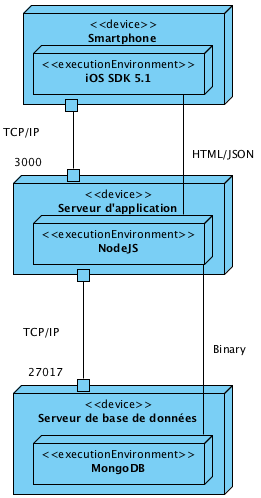
\includegraphics{diag_deploiement.png}
\end{center}

\section{Architecture des Composants en 5 couches} % (fold)
\label{sec:architecture_des_composants_en_5_couches}

L’application mobile est divisée en cinq couches de fonctionnalités, totalement autonomes les unes des autres, et communiquant par un système de file : chaque couche ne dialogue qu’avec les couches voisines supérieure et inférieure. Toutes les couches doivent agir de façon transparente les unes des autres. La séparation des couches est la suivante :

Couche Données : cette couche contient les données physiques stockées dans la base de données MongoDB. Elle ne requiert pas d’implémentation Objective-C particulière et fonctionne simplement comme un espace de consultation massif.

Couche Mapping : cette couche contient l’implémentation des accès à la base de données afin de la masquer à la couche métier.

Couche Métier : cette couche contient les objets métiers de l’application. Il existe un objet par fonctionnalité de l’application. Ces objets implémentent les fonctionnalités spécifiques relatives à la gestion du covoiturage, et font le lien entre la couche contrôleur et la couche mapping.

Couche Application : cette couche contient la partie fonctionnelle de l’application. Elle s’appuie sur les objets métier pour réaliser les actions sollicitées par l’utilisateur par l’intermédiaire de la couche présentation. Elle est en charge de vérifier la validité des requêtes de la couche présentation. Il existe un contrôleur par fonctionnalité de l’application. Le schéma utilisé est le MVC (Modèle Vue Contrôleur), mis en oeuvre en utilisant le framework Foundation d'Apple. Plus d’informations sont disponibles dans le paragraphe suivant.

Couche Présentation : cette couche représente les interfaces qui permettent de présenter les contenus générés par la couche présentation, grâce à des vues dynamiques. Elle se charge d’afficher des contenus à l’utilisateur et de lui offrir des interfaces avec la couche contrôleur pour interagir avec l’application.

\subsubsection{L'architecture MVC} % (fold)
\label{ssub:l_architecture_mvc}
Les couches présentation et application s’appuient  sur l’architecture « Modèle-Vue-Contrôleur » qui permet de séparer le fonctionnel de l’interface. Cette architecture est réalisée par une conjonction d’un contrôleur et d’un nombre quelconque de vues qui offrent le rendu à l’utilisateur. Les données calculées par le contrôleur et fournies aux vues pour être affichées sont les modèles. Le contrôleur s’appuie  sur les couches inférieures pour obtenir ces données.

L'utilisateur sollicite une action par l’intermédiaire d’une Vue. Cette action est transmise au contrôleur, qui en vérifie la validité et s’appuie sur la couche métier pour l’effectuer. Enfin le contrôleur renvoi sur la vue correspondant à la demande de l’utilisateur.

\chapter{Structure des données globales, des fichiers et des bases de données} % (fold)
  Les données sont centralisées dans une unique base de données MongoDB installée sur le serveur de base de données (les scripts de création des collections et des tuples de la base de données sont livrés avec l’application). Ces données sont utilisées par l’application GeoBBS.

\chapter{Stratégie de traitement des erreurs et des exceptions}
  Dans ce paragraphe sont exposées les différentes stratégies mises en place pour gérer les erreurs, i.e. empêcher l’application de s’effondrer sur n’importe quelle erreur et rendre les erreurs compréhensibles pour l’utilisateur.

\section{Stratégie d’exceptions par couches}
  Afin de permettre une gestion localisée des exceptions, il a été décidé que chaque couche prenne en compte. Ainsi, la couche mapping est en charge des exceptions lors des accès à la base. La couche contrôleur est en charge des exceptions dues au mauvais formatage des données et de transmettre des messages d’erreur textuels à la couche présentation pour l’utilisateur. De cette façon, chaque couche agit de façon autonome et la réutilisation des composants est possible.

\section{Vérification des données saisies}
  Une des principales sources d’erreurs dans les applications est due à des saisies erronées de la part de l’utilisateur. Ces erreurs peuvent être de plusieurs niveaux : erreurs de formatage, non suivi des règles métier, contraintes de base de données. Elles doivent être interceptées le plus tôt possible dans le cheminement de l’architecture afin d’une part que la logique soit respectée (chaque couche a un rôle particulier, il doit être  rempli sans supposer que d’autres couches le feront à sa place), et d’autre part que le nombre de traitements ne soit pas excessivement grand.

Les différents niveaux de vérifications de données sont les suivants :
\begin{description}
\item[couche contrôleur] : les formulaires des écrans sont validés. On peut alors vérifier que les données ne sont pas absentes, ou mal formatées. Ce sont des vérifications sans logique métier, simplement applicable à tout type de formulaire.
\item[couche métier] : une fois les valeurs saisies validées, la prochaine étape est de vérifier l’adéquation métier de ces données. Par exemple, une voiture apparaissant dans des mouvements ne peu pas être supprimée mais simplement retirée de la circulation. Ce genre de règles métiers doit être vérifiées par cette couche.
\item[couche mapping] : cette couche se charge de vérifier toutes les règles de gestion implémentées dans la base de données. Cela permet de passer au crible toutes les erreurs de saisies qui seraient soit mal gérées par les couches supérieures, soit appartenant à des cas très spécifiques d’erreurs. Notamment, la gestion des transactions est primordiale. La partie serveur se charge d’une grande partie de ces problématiques, il convient toutefois de définir les contraintes sur la base de données avec prudence et précision.
\end{description}

\section{Sécurisation des accès aux données}
  L'application serveur et mobile étant des prototypes et étant destiné à être testé dans un environnement protégé, il n'y a aucune sécurité.

\subsection{Justification des choix d'architecture, des composants et du langage}

  Les choix de l'architecture sont en partie imposés  par le maître d'ouvrage. Celui-ci préconise l'utilisation de MongoDB comme SGBD, ainsi que le langage Objective-C pour l'application mobile et CoffeeScript/JavaScript pour la partie serveur.

  GeoBBS a été développée selon une architecture 5 couches. Ce choix permet d'accroître l'indépendance et la réutilisation des composants. Ainsi pour chacune des couches, il est possible de changer le choix technique ou l'implémentation de façon transparente pour les autres couches. D'autre part le découpage en couche permet une plus grande réutilisation synonyme d'économie à terme. En contrepartie, il faut être conscient qu'une telle architecture réduit les performances générales du système du fait du cheminement indirect par les différentes couches. De plus, le primo investissement est plus lourd en terme de développement. Les économies se réalisent sur les extensions et la maintenance.

\chapter{Conception détaillée des composants}
\subsection{Système d’information}
\subsubsection{Règles de gestion}

  Les règles de gestion décrivent la nature des relations entre les entités d’un système d’information. L’ensemble de ces règles permet de définir un système correspondant à une problématique métier précisément adaptée aux besoins du client. Ces règles de gestion sont utilisées directement dans le modèle métier : chaque règle correspond à une relation  entre 2 (ou plusieurs) entités. Les entités métiers sont indiquées en italique.

\begin{description}
  \item[R1] un User peut créer plusieurs Check
  \item[R2] un User peut aussi être un Dev ou Dealer
  \item[R3] un Dev gère une et ou plusieurs applications
  \item[R4] un Dealer gère une ou plusieurs ShopPlace
  \item[R5] un Check concerne une Place
  \item[R6] une Place peut être soit une privatePlace, une ShopPlace ou une PublicPlace
  \item[R7] une ShopPlace peut avoir une ou plusieurs Offer
  \item[R9] une Application surveille un ou plusieurs Check
  \item[R10] un User peut installer une ou plusieurs Application
\end{description}

\subsubsection{Modèle Métier}
Les modèles métier suivants sont les modèles que nous avons mis en place côté serveur. S'agissant d'un prototype, seul les modèles User (Code. \ref{code:modelUser}) et Check (Code. \ref{code:modelCheck}) ont été nécessaire.

\begin{lstlisting}[float=htb, frame=lines, caption={Model User}, label={code:modelUser}]
class User

    # new User(login, password, ...)
    constructor: (@login = 'unknown'
                , @password = ''
                , @_id = new BSON.ObjectID()
                , @checks = []) ->

    # @chainable
    fromUser: (User) ->
      @_id = User._id
      @login = User.login
      @password = User.password
      @checks = User.checks

      @
\end{lstlisting}

\begin{lstlisting}[float=htb, frame=lines, caption={Model Check}, label={code:modelCheck}]
class Check
    # new Check(loc, User, ...)
    constructor: (@loc = {}
                  , User
                  , @opt = {}
                  , @_id = new BSON.ObjectID()) ->
      @_userId = if User && User._id then User._id else new BSON.ObjectID()

      @loc.lat = parseInt(@loc.lat, 10) || -1
      @loc.lon = parseInt(@loc.lon, 10) || -1

      @User = User.getGeneralInfo()
      @opt.date or= Date.now()
\end{lstlisting}


\subsection{Base de données}
Voici le modèle de notre base de données (Figure. \ref{fig:amqp1}) tel qu'il est prévu dans le projet finale.

\begin{figure}[htb]
  \centering
  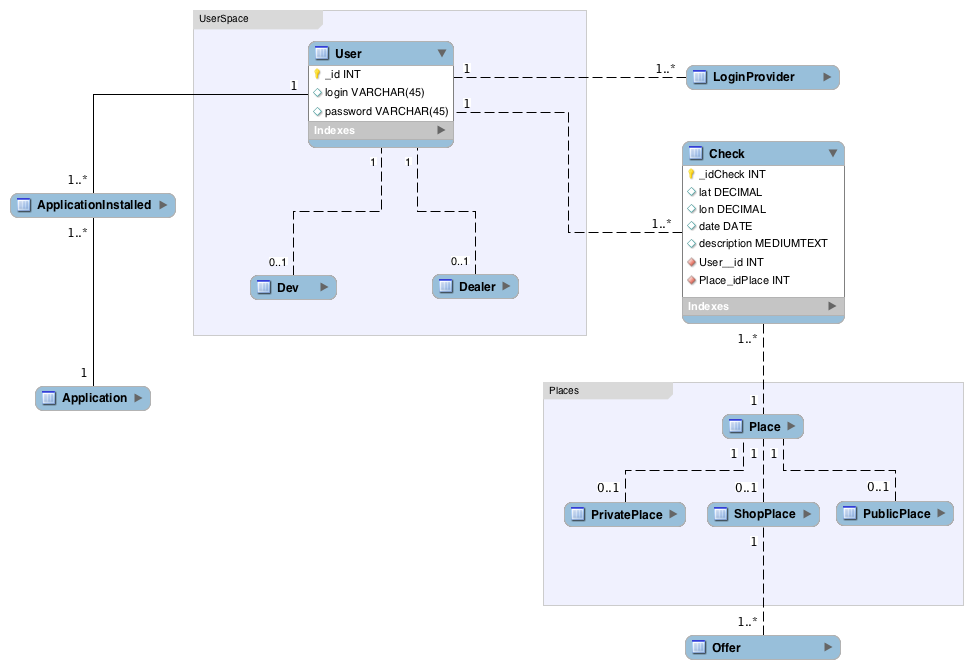
\includegraphics[width=\textwidth]{diagrameBDD/model.png}
  \caption{Base de données de la plateforme GeoBBS}
  \label{fig:amqp1}
\end{figure}

\chapter{Infrastructure GeoBBS}
\section{Architecture détaillée du composant}
L'application se divise en deux parties: une partie destinée à l'interconnexion avec la base de données: la partie serveur. Et une autre partie destiné à l'affichage et à l'interaction sur ces données: l'application mobile.

Le choix de l’architecture à 5 couches a été effectué. Nous allons dans les prochains paragraphes détailler le fonctionnement de chaque couche. Il est à noter que les couches Présentation et Contrôleur ont été développés en utilisant le paradigme MVC.


Pour mettre en œuvre cette architecture nous avons utilisé :
\begin{description}
  \item[MongoDB] pour la couche données
  \item[NodeJS] pour la couche physique
  \item[Apple Foundation Framework] pour la couche mapping, metier et application et présentation.
\end{description}

\subsection{Apple Foundation Framework}
  Apple Foundation Framework permet de mettre en œuvre facilement le paradigme MVC en limitant les dépendances entres Modèles, Vues et Contrôleurs. Foundation offre des types de base pour implémenter les contrôleurs et les modèles. De plus, il possède nativement un contrôleur central qui se charge de dispatcher les requêtes de la couche Présentation sur le contrôleur approprié. Enfin les opérations dites « génériques » inhérentes au modèle MVC sont réalisées par le framework.

\subsection{Couche Physique}
  La couche physique nécessite MongoDB pour sa mise en place. Elle a été modélisée par un Modèle Métier en utilisant Visual Paradigm. Ces diagrammes sont présentés plus haut. Le script de création de la base est disponible dans les sources. Il doit ensuite être exécuté dans la base de données. Un jeu de données de test est aussi mis en place sous forme d’un script chargé de remplir la base avec des données cohérentes pour tester l’application.
  
  La communication avec la couche physique se fait au moyen d’un driver NodeJS appelé MongoDb-native.

\subsection{Couche Mapping}
Cette couche est intégralement gérée par le framework de manière transparente.

\section{Couche Métier}
  La couche métier a comme rôle primordial de proposer un ensemble de services génériques sur les données, tout en faisant respecter les règles métier et les contraintes inhérentes au domaine d’activité.
  Il existe un objet métier pour chaque fonctionnalité de l’application. Les opérations les plus fréquentes sont les opérations CRUD : Create, Read, Update, Delete (Créer, Lire, Modifier, Supprimer). Ces opérations sont primordiales et doivent être l’ensemble minimal de méthodes fournies par toutes les entités. Elles font simplement le lien entre la couche Mapping et la couche Application.
  Ces opérations peuvent être bien plus que de simples CRUD, en intégrant par exemple de la logique métier spécifique au domaine de la géolocalisation. D’autres opérations spécifiques au métier sont aussi présentes quand cela est nécessaire.

\section{Couche Application}
Cette couche a pour rôle d’implémenter les cas d’utilisations qui seront présentés aux futurs bénéficiaires du système. L’architecture de la couche se base sur le modèle MVC expliqué plus tôt. Un contrôleur est mis en place pour chaque fonction de l’application. De plus, un intercepteur se charge de contrôler les accès, et un dispatcheur de renvoyer les requêtes sur le contrôleur approprié. Les contrôleurs sont en charge de :
\begin{itemize}
  \item vérifier que les données saisies sont correctes
  \item faire appel à la couche métier pour effectuer les traitements demandés
  \item placer dans le Model les données nécessaires à la couche présentation
  \item renvoyer l’utilisateur sur la couche présentation correspondant à sa demande
\end{itemize}

\section{Couche Présentation}
Toute la partie de présentation du projet GeoBBS est également gérée par le framework d'Apple qui propose un système de vue créé à l'aide d'Interface Builder.

\subsection{Sessions utilisateurs}
L’authentification d’un utilisateur conduit à l’ouverture d’une session qui permettra à celui-ci de naviguer sur toute l'application sans devoir s’identifier à chaque fois. La technologie employée pour la réalisation de l'application permet de définir une session utilisateur contenant un nombre quelconque de variables de sessions, définies et existantes pendant toute la durée de la session.

\subsection{Gestion interne de l’authentification}
Il convient de détailler les différents composants qui rentrent en jeu lors d’une authentification utilisateur. Lors de la soumission du formulaire d’identification par l’utilisateur, une première vérification est effectuée, permettant de s’assurer que ni le champ de mot de passe, ni le champ de login ne sont vides. Ensuite, les données sont comparées avec les données stockées en base :
\begin{itemize}
  \item Vérifier que le mot de passe correspond bien à l’utilisateur
  \begin{itemize}
    \item Dans le cas où le mot de passe est erroné, rediriger vers le formulaire avec une notification d’erreur
    \item Dans le cas où le mot de passe est correct, charger les droits de l’utilisateur et rediriger vers la page d’accueil de l’application.
  \end{itemize}
\end{itemize}

\subsection{Gestion des droits d’utilisateurs}
Au sein de la plateforme, il existe plusieurs catégories d’utilisateurs qui n’ont pas accès aux mêmes fonctionnalités. Les groupes d’utilisateurs considérés sont les suivants :
\begin{itemize}
  \item Administrateur de la plateforme
  \item Utilisateur de la plateforme
  \item Développeur d'application
  \item Gestionnaire de boutique.
\end{itemize}

  \end{onehalfspace}
\end{document}